\documentclass[a4paper]{article}

\usepackage[margin=2.5cm]{geometry}
\usepackage[pdftex]{graphicx}
\usepackage[utf8]{inputenc}
\usepackage[T1]{fontenc}
\usepackage{textcomp}
\usepackage{babel}
\usepackage{amsmath, amssymb}
\usepackage[colorlinks=true,linkcolor=blue]{hyperref}
\usepackage{float}
\usepackage{mathrsfs}
%\usepackage{enumitem}
%% for identity function 1:
%\usepackage{bbm}
%%For category theory diagrams:
%\usepackage{tikz-cd}
%%For code (e.g. python) in latex:
%\usepackage{listings}
%
%Usage: 
%\begin{lstlisting}[language=Python]
%\end{lstlisting}

\newcommand{\incfig}[2][1]{%
\def\svgwidth{#1\columnwidth}
\import{./figures/}{#2.pdf_tex}
}


% figure support
\usepackage{import}
\usepackage{xifthen}
\pdfminorversion=7
\usepackage{pdfpages}
\usepackage{transparent}

\pdfsuppresswarningpagegroup=1

\setlength\parindent{0pt}

\newcommand{\qed}{\tag*{$\blacksquare$}}
\newcommand{\qedwhite}{\hfill \ensuremath{\Box}}

%Inequalities
\newcommand{\cycsum}{\sum_{\mathrm{cyc}}}
\newcommand{\symsum}{\sum_{\mathrm{sym}}}
\newcommand{\cycprod}{\prod_{\mathrm{cyc}}}
\newcommand{\symprod}{\prod_{\mathrm{sym}}}

%Linear Algebra

%Redeclaring Span and image
\DeclareMathOperator{\Span}{span}
\DeclareMathOperator{\Ima}{Im}
\DeclareMathOperator{\diag}{diag}
\DeclareMathOperator{\Ker}{Ker}
\DeclareMathOperator{\ob}{ob}


%Row operations
\newcommand{\elem}[1]{% elementary operations
\xrightarrow{\substack{#1}}%
}

\newcommand{\lelem}[1]{% elementary operations (left alignment)
\xrightarrow{\begin{subarray}{l}#1\end{subarray}}%
}

%SS
\DeclareMathOperator{\supp}{supp}
\DeclareMathOperator{\Var}{Var}

%NT
\DeclareMathOperator{\ord}{ord}

%Alg
\DeclareMathOperator{\Rad}{Rad}
\DeclareMathOperator{\Jac}{Jac}

\DeclareMathAlphabet{\pazocal}{OMS}{zplm}{m}{n}
\newcommand{\unif}{\pazocal{U}}

\begin{document}











    \textbf{1.3.6:} Let
    $\tilde{X}$ be the covering space shows and
    consider any one of the basepoints
    $p^{-1}(x_0)$ where $x_0 = (0,0)$ in $X$.\\
    Consider this basepoint to be $0$ 
    and each subsequence basepoint in the fiber
    of $0$ to be $1,2,3,$ etc. and preceeding basepoints
    $-1, -2, \ldots$. Now let the outermost
    circle of radius $1$ in each copy of the Hawaiian earring
    unfold to the linesegments
    between these integers. I.e. we place each
    copy of the earrings onto each integer and unfold
    the outmost circle to connect the components.\\
    Let  $p$ be the covering map that
    collapses this covering space such that
    each of the circles $C_n$ is mapped to the
    $C_n$ in $X$ and each segment $\left[ n,n+1 \right] $ 
    is mapped to $C_1$.
    This is a covering map since for any $x$ that is not on $C_1$, we can find a neighborhood around this point
    that does not intersect $C_1$, and the preimage of this neighborhood
    will simply be the collection of identical neighborhood each of which
    is homeomorphic to the neighborhood in $X$ by the identity
    . For any point on  $C_1$ that is not the basepoint,
    its preimage will be of the form $x' + \mathbb{Z}$, and we
    can find a neighborhood that also only intersects $C_1 - \left\{ x_0 \right\} $ and
    whose image will be the collection of some open intervals
    $I + \mathbb{Z}$ where each $I$ is clearly homeomorphic
    to the neighborhood on $X$ by $z \to e^{2 \pi i z}$.\\
    For $x_0$ whose fiber is $\mathbb{Z}$, we can
    choose a neighborhood that does not cover $C_1$ whose
    preimage will then not contain some
    $k + \mathbb{Z}$ for some $ k \in (0,1)$. The components
    will therefore be disconncted and each will be homeomorphic
    to the neighborhood by the identity. So this is a 
    covering space.\\
    \linebreak
    Now let $\tilde{\tilde{X}}$ denote the covering space
    obtained by first taking a copy of $\tilde{X}$ and
    then connecting each component (i.e. 
    a specific chosen $[n,n+1)$ and  $\bigcup_{i \in \mathbb{N}} C_{n,i}$ 
    where $C_{n,i}$ is the circle of radius $i$ centered at
    the integer $n$) to its corresponding component
    in the copy by deforming the circles
    $C_{k,k}$ into a line segment connecting the copies of
    integer the integer  $k$. Let
    $p'$ be the covering map that collapses $\tilde{\tilde{X}}$ 
    to $\tilde{X}$ as one would expect (mapping the
    copy of $\mathbb{R}$ to $\mathbb{R}$ and each
    circle to each circle - the circles $C_{k,k}$ also to
    its copy.\\
    \linebreak
    Checking that $p'$ is a homeomorphism is done equivalently
    to $p$; in this case, for any integer  $n$, we choose
    a neighborhood that does not contain $C_{n,n}$ nor
    any other integers, and hence its preimage
    will be two components, each homeomorphic to itself by the identity.\\
    \linebreak
    Now the composition of $p \circ p'$ is not a covering map:
    take any neighborhood of $x_0 = (0,0)$. This
    neighborhood will contain some $C_k$ for $k \in \mathbb{N}$,
    and thus its preimage under $p\circ p'$ will contain
    the linked copies of the earrings of $k$ which
    is not a homeomorphism under $p \circ p'$ as it is not injective
    on the disjoint components.\\

\begin{figure}[h]
    \centering
    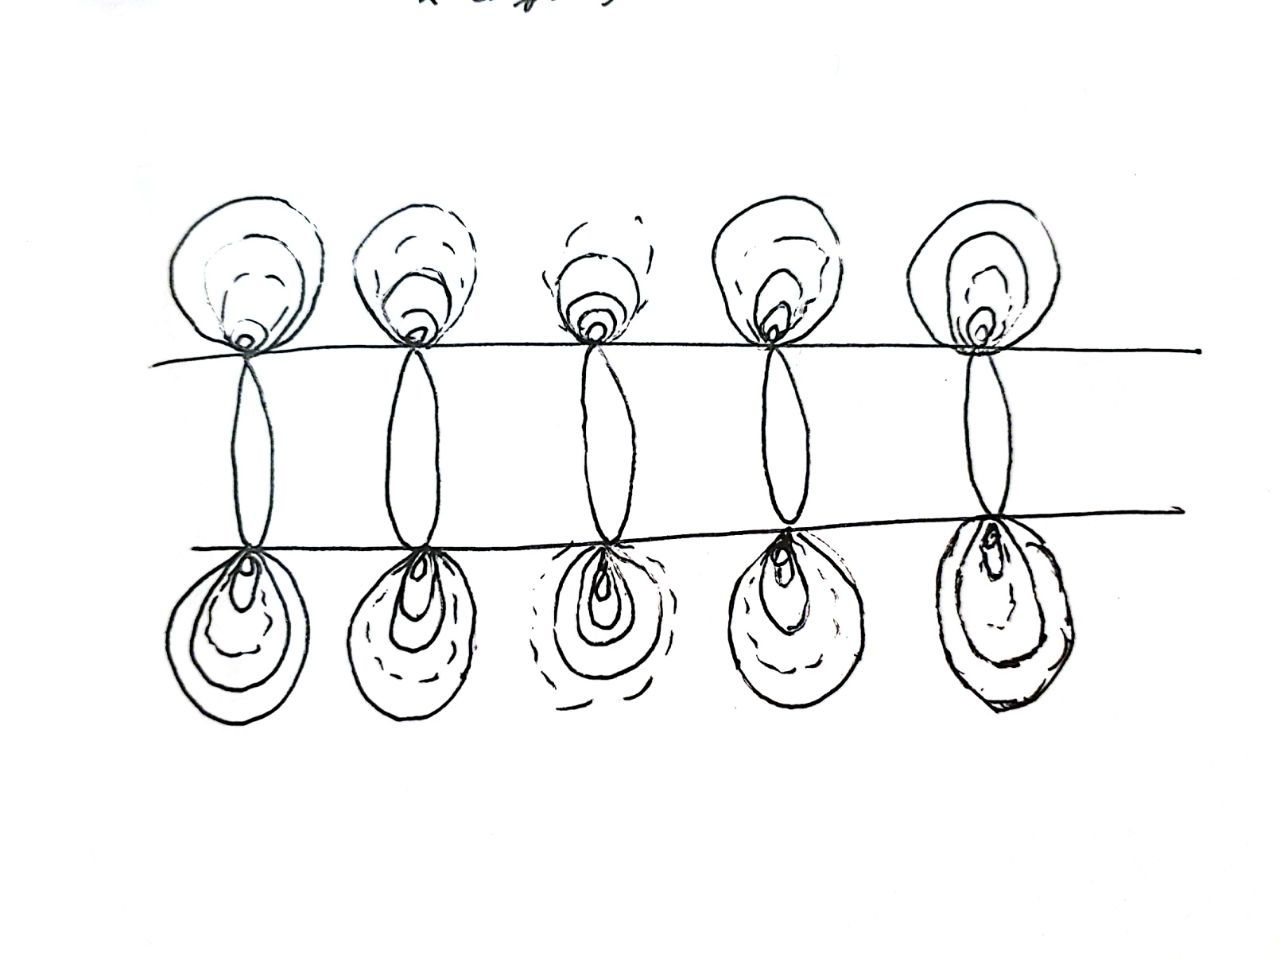
\includegraphics[width=0.8\textwidth]{1.jpg}
    \label{fig:1-jpg}
\end{figure}



    \linebreak
    \textbf{1.3.14:} 

    From p. 78, we have that $\mathbb{R}P^2 \vee \mathbb{R}P^2$ is the orbit
    space for the Cayley complex of $G = \mathbb{Z}_2 * \mathbb{Z}_2
    = \langle a,b  \mid a^2, b^2 \rangle$, depicted on p. 78 as an infinite
    string of 2-spheres linked at points as follows:

\begin{figure}[htpb]
    \centering
    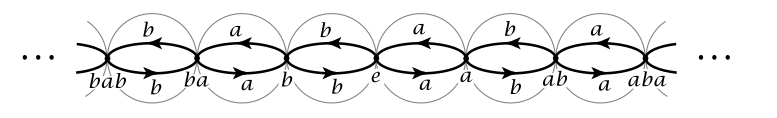
\includegraphics[width=0.8\textwidth]{orbit-space.png}
    \label{fig:orbit-space-png}
\end{figure}

The action on this space is as follows: elements of any subgroup generated by $ab$
act on $\tilde{X_G}$ by
translations by an even number of units, while each remaining element of
$\mathbb{Z}_2 * \mathbb{Z}_2$ acts by an antipodal map on one of the spheres
and flips the chain end-for-end about the sphere.\\
This action satisfies $(*)$ on page 72 since it is clear that if we choose any
point on the chain, then this point gets mapped to each copy of its point and
each copy of its antipodal point by exactly one element of $g$; hence any small
neighborhood around the point restricted to that hemisphere or side of the
equator works for $(*)$. Since it is a covering space action, we can use
proposition 1.40 to deduce that that quotient map
$p : \tilde{X_G} \to X_G = \mathbb{R}P^2 \vee \mathbb{R}P^2$ is a normal
covering space and by the remark on page 77, it is in fact a universal cover of
$\mathbb{R}P^2 \vee \mathbb{R}P^2$, thus corresponding to 
$\langle a,b  \mid a^2, b^2 \rangle$.\\
\linebreak
By playing around with the group we find that the subgroups are of the
following forms:\\
\textbf{1:} The group itself $G$.\\
\linebreak
\textbf{2:} Subgroups of the form
$\langle (ab)^{n} \rangle$ or $\langle (ba)^{n} \rangle$.\\
\linebreak
\textbf{3:} Subgroups of the form
$\langle (ab)^{n}a \rangle$ or $\langle  (ba)^{n} b \rangle$.\\
\linebreak
\textbf{4:} Subgroups of the form
$\langle (ba)^{n} b, (ba)^{m}  \mid n < m \rangle $ and 
$\langle  (ab)^{n} a, (ba)^{m}  \mid n < m \rangle$.\\
\linebreak

By proposition 1.40.(c), each of these types of
subgroups is isomorphic to the fundamental group the orbit
space
of $\tilde{X_G}$ under the action induced by a generator of the subgroup.\\
\linebreak
For the trivial subgroup, we get the Cayley complex as shown above.\\
\linebreak
For subgroups of type two we get, by modding out,
$2n$ spheres and we link the end circles by a loop at the attaching points.\\
\linebreak
For subgroups of type three, we get an infinite chain of 2-spheres extending
as shows in the picture from the basepoint $e$, onto which $\mathbb{R}P^2$ is
attached at one end. To get the other type three subgroup, we exchange each
copy of $a$ for $b$ and $b$ for $a$.\\
\linebreak
For subgroups of type three, we get a finite chain as shown where two copies of
$\mathbb{R}P^2$ have been attached at either end. 
    


\begin{figure}[h]
    \centering
    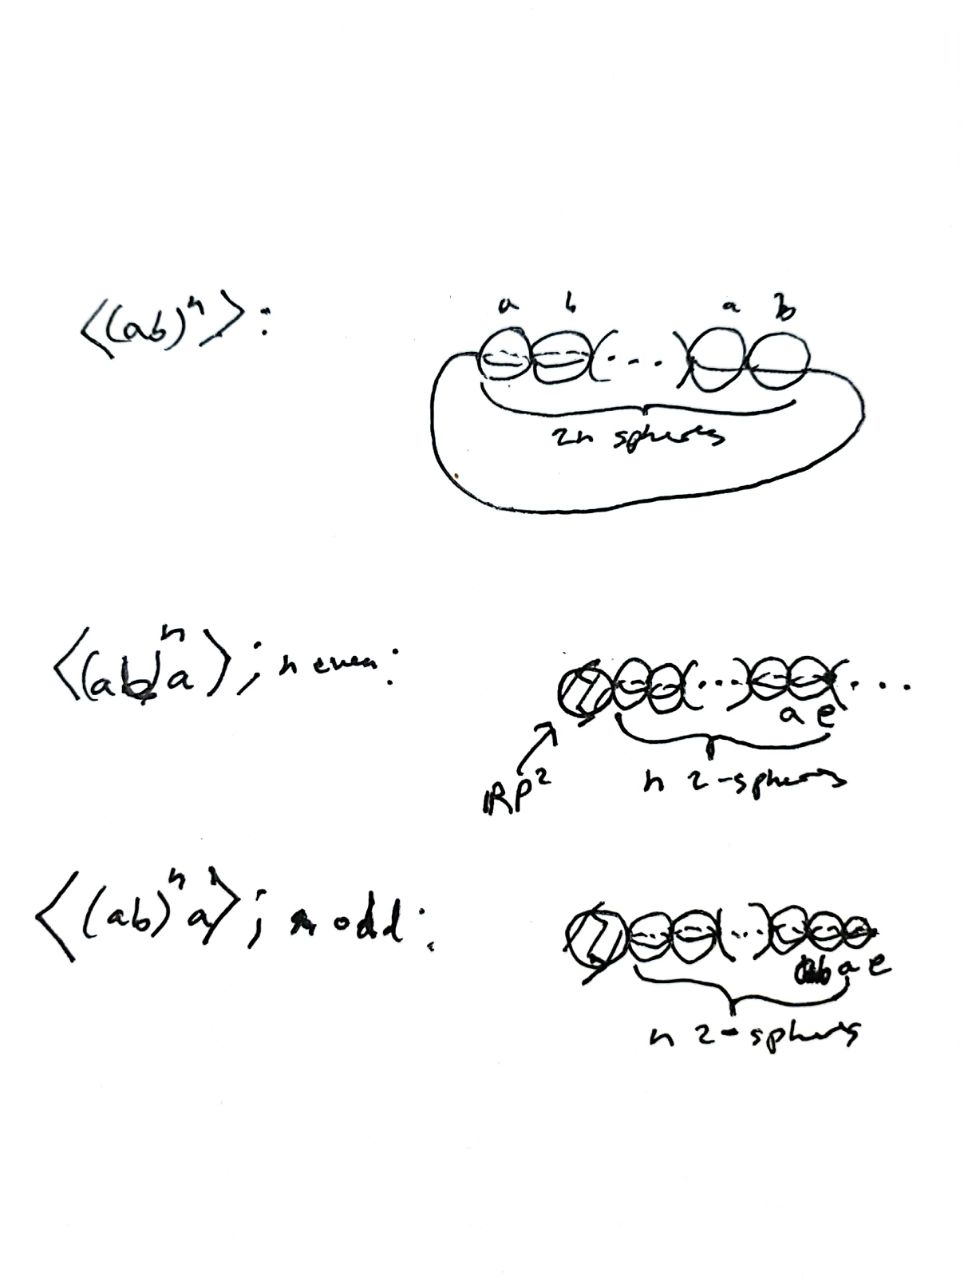
\includegraphics[width=0.8\textwidth]{22.jpg}
    \label{fig:22-jpg}
\end{figure}

\begin{figure}[h]
    \centering
    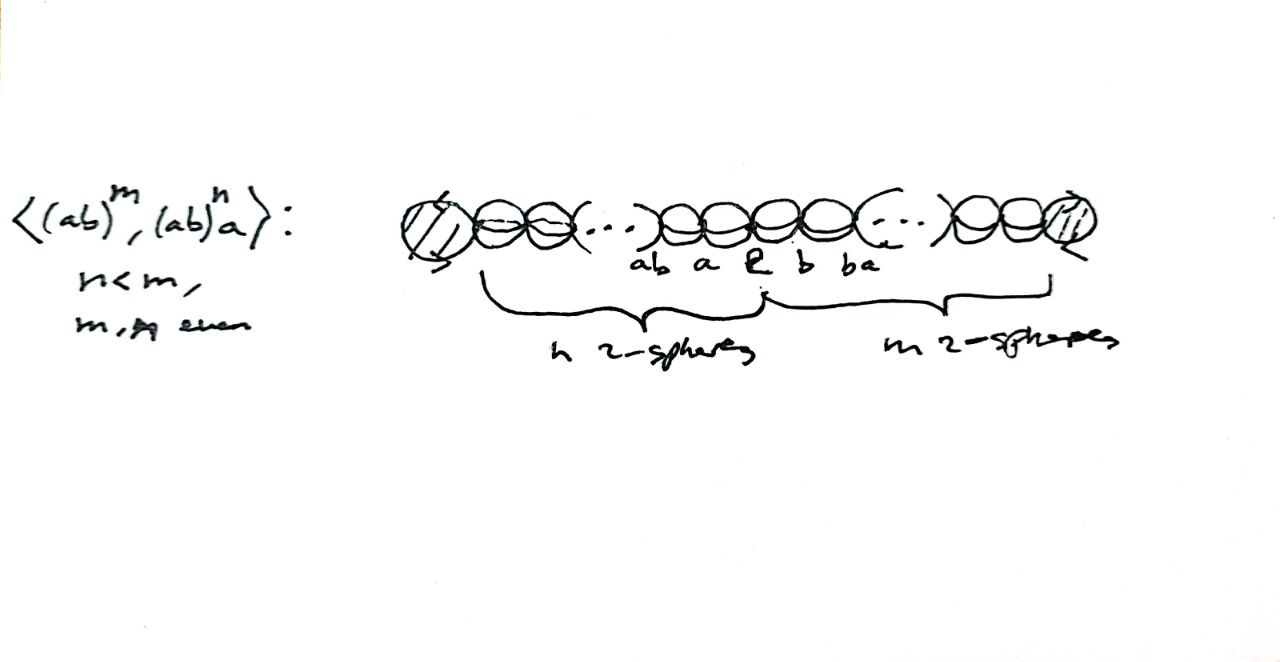
\includegraphics[width=1\textwidth]{21.jpg}
    \label{fig:21-jpg}
\end{figure}





\end{document}
